\section{Problem (8)}
	The \cref{fig:hw9_problem8} shows a three-particle-system, with masses $m_{1} = \ 2.8 \ kg$, $m_{2} = \ 4.0 \ kg$, and $m_{3} = \ 9.6 \ kg$.

	\begin{figure}[H]
		\begin{center}
			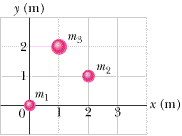
\includegraphics[scale=1]{hw9_problem8}
			\caption{Illustration of Problem 8}
			\label{fig:hw9_problem8}
		\end{center}
	\end{figure}

	\subsection{Question (a)}

		What is the $x$ coordinate of the system's center of mass?

		\textbf{R:}

		\begin{align}
			X_{CM} = &\frac{\displaystyle\sum_{i=1}^{3} m_i x_{i}}{\displaystyle\sum_{i=1}^{3} m_i}& \notag \\
			= &\frac{(2.8 \ kg)(0) + (4.0 \ kg)(2 \ m) + (9.6 \ kg)(1 \ m)}{(2.8 \ kg) + (4.0 \ kg) + (9.6 \ kg)}& \notag \\
			= &\frac{17.6 \ kg \times m}{16.4 \ kg}& \notag \\
			= &1.\overline{0731} \ m&
		\end{align}

	\subsection{Question (b)}

		What is the $y$ coordinate of the system's center of mass?

		\textbf{R:}

		\begin{align}
			Y_{CM} = &\frac{\displaystyle\sum_{i=1}^{3} m_i y_{i}}{\displaystyle\sum_{i=1}^{3} m_i}& \notag \\
			= &\frac{(2.8 \ kg)(0) + (4.0 \ kg)(1 \ m) + (9.6 \ kg)(2 \ m)}{16.4 \ kg}& \notag \\
			= &\frac{23.2 \ kg \times m}{16.4 \ kg}& \notag \\
			= &1.\overline{41463} \ m&
		\end{align}
